\documentclass{assignment}
\usepackage{graphicx}
\usepackage{parskip}

\class{Βιομηχανική Ηλεκτρονική}
\assignment{Σειρά Ασκήσεων 1}

\begin{document}

\maketitle

Παρακάτω παρατίθεται το σχεδιάγραμμα όπως λήφθηκε απο το \en{Pspice}.
Ως πηγή χρησιμοποιήθηκε ημιτονοειδής πηγή με μέτρο $V_{AMPL} = 220 * \sqrt{2} \simeq 311$.

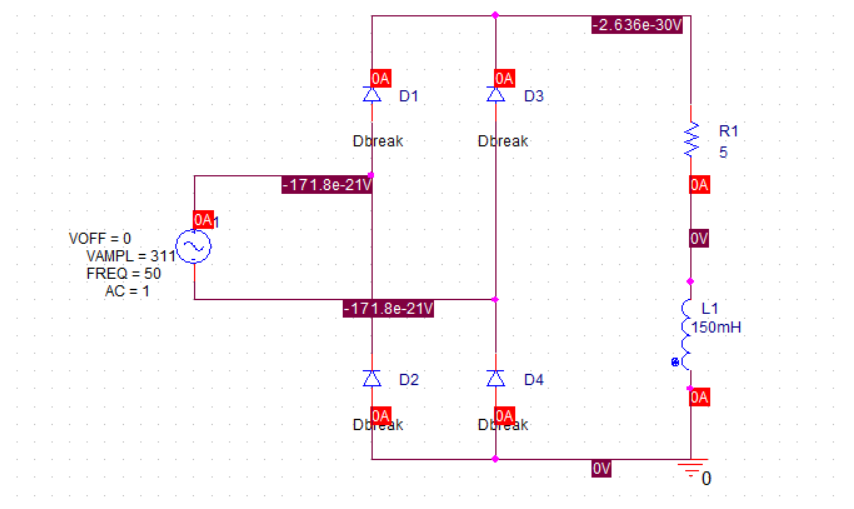
\includegraphics[width=0.7\textwidth]{exercise1-diag} 

Τοποθετόντας τα κατάλληλα \en{markers} στις ζητούμενες θέσεις παίρνουμε 
τις ακόλουθες κυμματομορφές της τάσης και ρεύματος εισόδου και εξόδου.

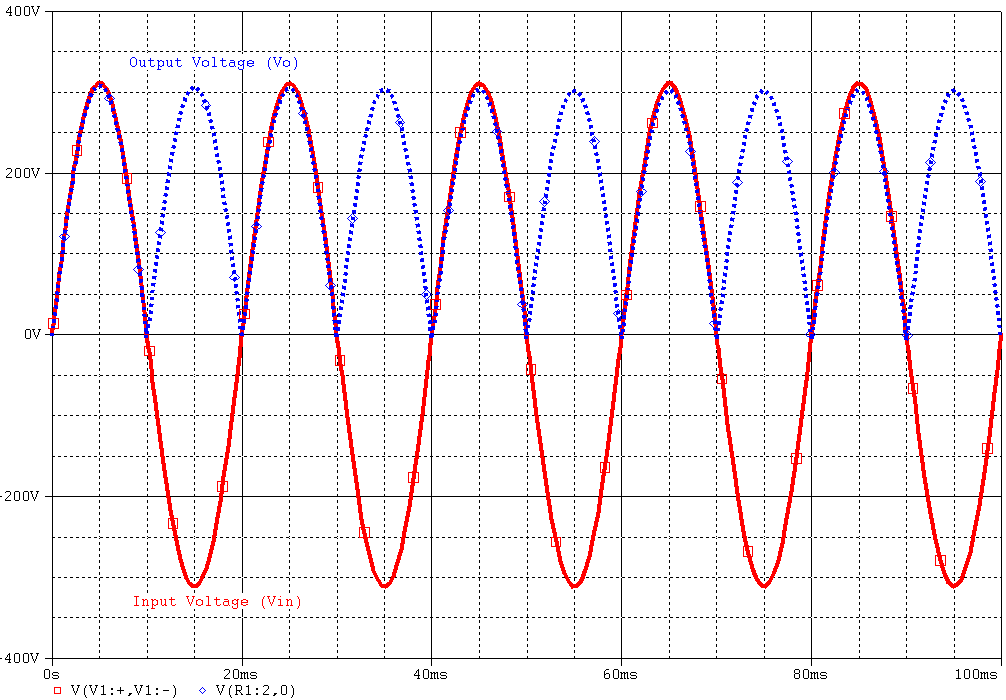
\includegraphics[width=0.45\textwidth]{exercise1-1} 
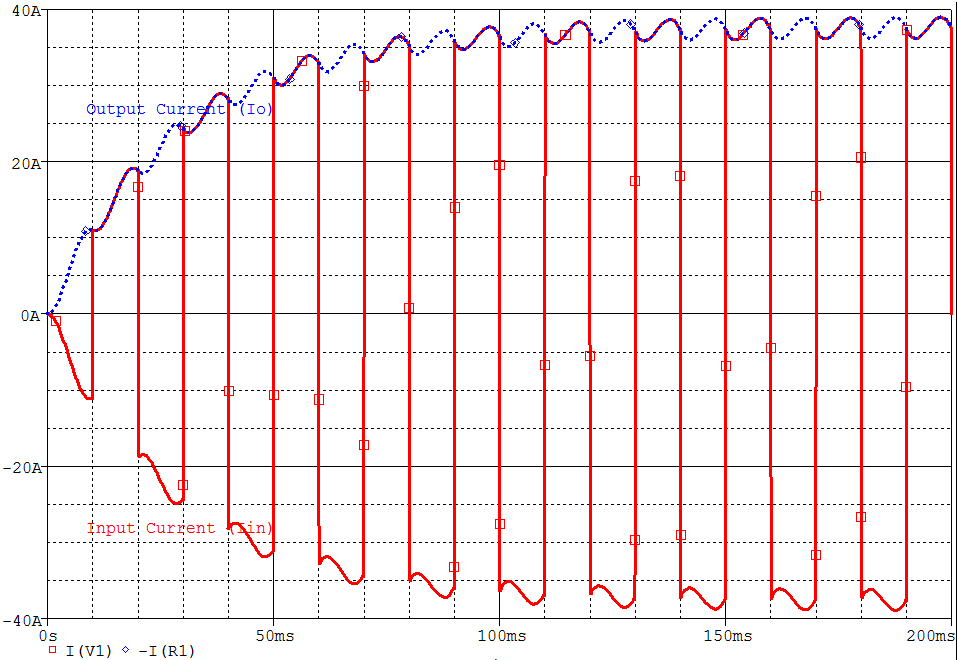
\includegraphics[width=0.45\textwidth]{exercise1-2}


Με τη προσθήκη \en{trace} ρεύματος δια $\sqrt{2}$, μετράμε την \en{RMS} τιμή του ρεύματος εξόδου ως $I_{o_{rms}} \simeq 27.4$\en{A}.\\
Η φαινομενική ισχύς υπολογίζεται πολλαπλασιάζοντας την \en{RMS} τάση και ρεύμα εξόδου, επομένως $S \simeq 6028$\en{VA}.\\
Τέλος, χρησιμοποιόντας \en{trace} με τη συνάρτηση \en{AVG}, μετράμε προσεγγιστικά την μέση τάση εξόδου ως $\left<V_{o}\right> \simeq 188.4V$ και 
το μέσο ρεύμα εξόδου ως $\left<I_{o}\right> \simeq 37.3A$. 

\end{document}


